\setlength\intextsep{1mm}

\section*{\textbf{Introduction}}

\textbf{1.} Primary analysis on the Titanic dataset.

The given dataset was collected from the famous tradgic sinking of the Titanic ship, one of the largest ships at that time. We are given the training dataset (traing.csv) and testing dataset (testing.csv), which curated information of the passenger, including their names, Pclasses, sexes, ages, siblings, parches, ticket numbers, fares, cabins and embark locations. The training set also include a "Survived" column, indicating labels or targets of the samples, which is also the prediction goal for the given testing dataset.

\textbf{The goal of this project is to use the training data, clean it and train a two-class classifier to best predict whether passengers in the test dataset could survive or not. Also, another goal is to provide reasonings for model selection, traning details and the final sights from the trained optimized model.}

First of all, given the training and testing data, below is the statiscs about missing values in the datasets:
\begin{table}[H]
    \centering
    \begin{tabular}{|c|c|c|c|c|}
        \hline 
        Feature    &total       &unique values  &numb. of missing  &numb. of real   \\
        \hline
        PassengerId &891         &891         &0           &891             \\
        Survived    &891         &2           &0           &891             \\
        Pclass      &891         &3           &0           &891             \\
        Name        &891         &891         &0           &891             \\
        Sex         &891         &2           &0           &891             \\
        Age         &891         &88          &177         &714             \\
        SibSp       &891         &7           &0           &891             \\
        Parch       &891         &7           &0           &891             \\
        Ticket      &891         &681         &0           &891             \\
        Fare        &891         &248         &0           &891             \\
        Cabin       &891         &147         &687         &204             \\
        Embarked    &891         &3           &2           &889             \\
        \hline
    \end{tabular}
    \caption{Statistics of the training data}
    \label{statistics of the training data}
\end{table}

\begin{table}[H]
    \centering
    \begin{tabular}{|c|c|c|c|c|}
        \hline 
        Feature    &total       &unique values  &numb. of missing  &numb. of real   \\
        \hline
        PassengerId &418         &418         &0           &418               \\         
        Pclass      &418         &3           &0           &418               \\         
        Name        &418         &418         &0           &418               \\         
        Sex         &418         &2           &0           &418               \\         
        Age         &418         &79          &86          &332               \\         
        SibSp       &418         &7           &0           &418               \\         
        Parch       &418         &8           &0           &418               \\         
        Ticket      &418         &363         &0           &418               \\         
        Fare        &418         &169         &1           &417               \\         
        Cabin       &418         &76          &327         &91                \\         
        Embarked    &418         &3           &0           &418               \\ 
        \hline
    \end{tabular}
    \caption{Statistics of the testing data}
    \label{the training data}
\end{table}

As we can see from the above tables, about 20\% \textbf{Age} data is missing in both the training and testing dataset; majority (~77\%) of the \textbf{Cabin} data is missing in both datasets; 2 samples in the training set miss the \textbf{Embarked} data; and finally 1sample in the testing set miss the \textbf{Fare} data. Besides, some features are non-numerical data. Therefore, prior to our model training, we need to first deal with those missing data, and also apply feature transform/enginerring techniques if needed.


\section*{\textbf{Methodology}}

\textbf{1.} Data pre-processing. 
First of all, passenger's \textbf{Name} and \textbf{Ticket}, based on our intuitive, could hardly in any aspect be important for our prediction of survivals. Also the \textbf{Cabin} has a lot of missing values. Thus, those three features are directly deleted. 

To design the corresponding processing strategy for the rest of the features, I did an anlysis of the data type and value range first, as listed in the Table 3.
\begin{table}[H]
    \centering
    \begin{tabular}{|c|c|c|c|}
        \hline 
        col name    &Pre-processing                     &Initial Range  &Final Range    \\
        \hline
        Survived    &N/A                                &\{0, 1\}       &\{0, 1\}         \\
        Pclass      &N/A                                &\{1, 2, 3\}    &\{1, 2, 3\}      \\
        Sex         &Binary                             &\{male, female\}       &\{0, 1\}         \\
        Age         &Impute with median ; MinMaxScaler  &[0, 80]    &[0, 80]        \\
        SibSp       &N/A                                &\{0, 1, 2, 3, 4, 5, 8\}    &\{0, 1, 2, 3, 4, 5, 8\}\\
        Parch       &N/A                                &\{0, 1, 2, 3, 4, 5, 6\}    &\{0, 1, 2, 3, 4, 5, 6\}\\
        Fare        &Impute with median, MinMaxScaler   &[0, 512]   &[0, 1]    \\
        Embarked    &                                   &{C, Q, S}  &One-hot encoding    \\
        \hline
    \end{tabular}
    \caption{Data analysis and preprocessing strategy for each column}
    \label{Data preprocessing}
\end{table}

Among the listed feature, passengers'  \textbf{Sex} and \textbf{Embarked} are not numerical data, whereas the fares, Pclasses, ages and siblings are numerical. For convenience and consistency, in the data preprocessing step, the training set and the testing set are merged after removed the \textbf{survival} column in the training set.

Below are my reasonings for choosing the preprocessing strategy for each feature:

\begin{itemize}
    \item The \textbf{Sex} data is basically binary -- we could use 1 and 0 for male and female passengers respectively.
    \item The \textbf{Age} data also has ~20\% missing data and \textbf{Embarked} has 2 missing data. Using median value seems to be a reasonable choice to minimize the imputation effect to the overall distribution.
    
        \begin{figure}[H]
            \centering
            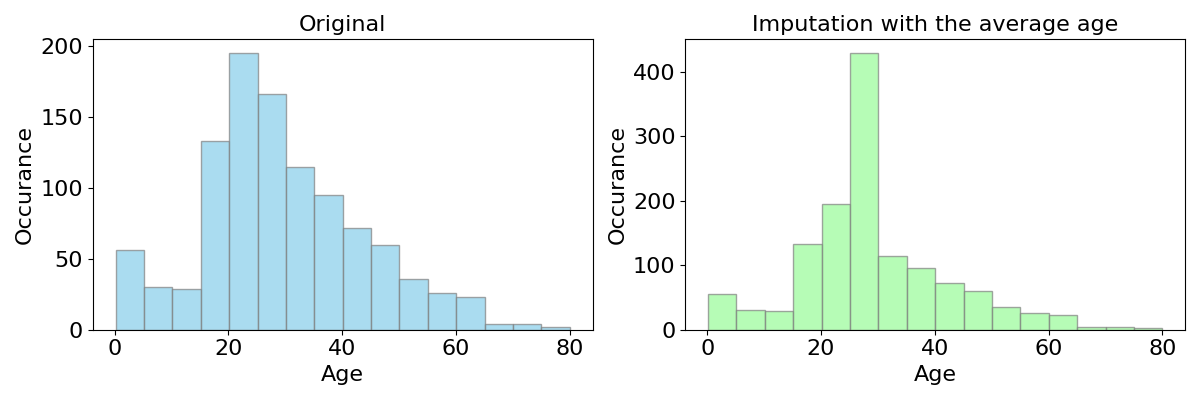
\includegraphics[width=160mm]{imputation_age.png}
            \caption{Imputing the Age data in the training set}
            \label{imputation of the age data}
        \end{figure} 

    \item The \textbf{Embarked} has three non-numerical catagories. Here, I used the one-hot encoding method, i.e., (1, 0, 0) for C, (0, 1, 0) for Q and (0, 0, 1) for S.
    \item Finally, the \textbf{Age} and \textbf{Fare} have one or two-orders of magnitude than other features. In order to have a smoothier training and faster convergence, I choose to use MinMax normalization to scale the original data to the range of [0, 1].
\end{itemize}

\textbf{2. Splitting the original training set to form the $Testing_{actual}$}
Since we do not have the true label for the testing sample in \textbf{test.csv}, I took \textbf{20\%} of my training set to form a real \textbf{testing set} whose labels are given. I denote this testing set as my actual testing set $Testing_{actual}$.


\textbf{3.} Details of implementations of models, including model initialization, hyperparameters tuning, and cross validation.

According to the rubric, three models, fixed shape universal approximator with kernel method, neural network method and tree-based method, should be trained. My models and also hyperparameters tuning strategies are listed in the following table. 

For \textbf{moel initialization}, at least three random seeds were tested and eventually picked the one that perform the best, though in most cases, their performances are all similarly. Using random seed means the initialization of all models is random to avoid the risk of reaching arbitary global minimum when initializing using all zero values. 

During searching the hyperparameters using grid search, each hyperparameter combination will traing a model and output the average cross-validation accuracy, as well as \textbf{the testing accuracy} on the \textbf{$Testing_{actual}$} mentioned above.

\begin{table}[H]
    \centering
    \begin{tabular}{|c|c|c|c|}
        \hline 
        Model       & hyperparameters & grid search & tuning strategy \\
        \hline
        \multirow{3}{*}{SVM kernel method}   &  Kernel & RBF & \multirow{3}{*}{5-fold cross-validation } \\
                                              &  Regularization parameter (C)  & \{0.1, 1, 10\}  &        \\
                                              &  Kernel coefficient (gamma)  & \{'scale', 'auto', 0.1, 1\}  &     \\ 
        \hline
        \multirow{4}{*}{Neutral Network} & hidden\_layer\_sizes  & (10,), (15,), (20,), (5, 10) & \multirow{4}{*}{5-fold cross-validation} \\
                        & regularization parameter ($\alpha$)   & \{0.0001, 0.001\} & \\
                        & learning\_rate\_init & \{0.1, 0.01\}& \\
                        & max\_iter & \{500\} & \\
        \hline
        \multirow{4}{*}{Random Forest}   &  n\_estimators & \{50, 100\} & \multirow{4}{*}{5-fold cross-validation} \\
                                              &  max\_depth  & \{None, 2, 5\}  &        \\
                                              &  min\_samples\_split  & \{2, 4, 6\}  &     \\
                                              & min\_samples\_leaf & \{1, 2, 4\} & \\
 
        \hline
    \end{tabular}
    \caption{Data analysis and preprocessing strategy for each column}
    \label{Model selection and hyperparameters tuning strategies}
\end{table}

The sklearn package was used to call all the three method in the Table 4.For each method, there are many hyperparameters that we could theoretically try. The middle column shows the hyperparameters I chose to tune for each method. And the third column shows the settings for each hyperparameter in the \textbf{grid search} process.

Explanations about the selections of hyperparameters are listed below:
\begin{itemize}
    \item \textbf{SVM kernel method: } The Radial Basis Function (RBF) kernel was used and it is a popular choice among kernel methods. Regulaization parameter (C) controls the tradeoff between having a smooth decision boundary and reaching high classification accuracy, a large C means allowing the decision boundary to be more complex in order to have more correct classification, whereas a small C means to have a more smoothier boundary. Lastly, the Kernal coefficient (gamma) is an internal parameter of the RBF kernel, which controls how far the influence of each datapoint can reach: a low value of gama means to have a far influence whereas a large value means to have a near influence. The C and gamma controls largely the performance of SVM kernel model and thus are chosen to be tuned.
    \item \textbf{Neural network: } Four hyperparameters are important in this model: hidden layer size (number of nodes in a hidden layer), regularization parameter ($\alpha$, the regularization factor in l2 normalization), learning rate, and maximum iterations. The hidden layer size defined the neural network architecture, and regularization parameter can help to avoid overfitting. Learning rate and maximum are important for model training and reach convergence.
    \item \textbf{Random forest: } Four hyperparameters are important in random forest: number of trees (n\_estimators), maximum depth of each tree (max\_depth), The minimum number of samples (min\_samples\_split) is the number required to split an internal node. Larger values prevent the model from creating nodes that represent small subsets of the data, potentially reducing overfitting. The minimum number of samples (min\_samples\_leaf) required to be at a leaf node. Similar to min\_samples\_split, larger values help prevent the creation of nodes with very few samples. The last three parameters can help avoid overfitting since the tree method is generally very easy to overfit.
\end{itemize}

The best hyperparameter set for each method was finally decided based on the cross-validation accuracy and testing accuracy on $Testing_{actual}$. Then, the hyperparameters were used to train a final model using the whole training set including the $Testing_{actual}$. Those final models were then used to predict the samples in the test.csv from the kaggle website.

\section*{\textbf{Results}} 

Based on the cross-validation accuracy and testing accuracy on $Testing_{actual}$, which was spliited from the intial training set. The table below listed the best hyperparameter sets for each model:

\begin{table}[H]
    \centering
    \begin{tabular}{|c|c|c|c|c|}
        \hline 
        Model       & hyperparameters & Best combination  & Val. Acc. & Test. Acc. \\
        \hline
        \multirow{3}{*}{SVM kernel method}   &  Kernel & RBF   & \multirow{3}{*}{79.6\%} & \multirow{3}{*}{88.8\%} \\
                        &  Regularization parameter (C)  &  10   &   & \\
                        &  Kernel coefficient (gamma)  &  0.1    &   & \\ 
        \hline
        \multirow{4}{*}{Neutral Network} & hidden\_layer\_sizes  & 15 & \multirow{4}{*}{79.9\%} & \multirow{4}{*}{87.7\%}\\
                        & regularization parameter ($\alpha$)   & 0.0001 &  & \\
                        & learning\_rate\_init & 0.1 & & \\
                        & max\_iter & 500  & & \\
        \hline
        \multirow{4}{*}{Random Forest}   &  n\_estimators & 50  & \multirow{4}{*}{83.0\%} & \multirow{4}{*}{88.2\%}\\
                        &  max\_depth  & None      &   & \\
                        &  min\_samples\_split  & 2     &  & \\
                        & min\_samples\_leaf & 1  & & \\
        \hline
    \end{tabular}
    \caption{The best hyperparameters}
    \label{the hyperparameter tuning}
\end{table}

The performance of each model on the $Testing_{actual}$ was used to pick up the best model from those three methods. The following plots summarize the performance of  models of each of those three methods using different hyperparameter combinations. The best combinations have already been summarized in the Table 5. 

To gain insights from these trained models, feature importance evaluation was performed for the best models from all three methods, using either the permutation\_importance method in sklearn or the build-in importance matrics (in the random forest model).

\begin{figure}[H]
    \centering
    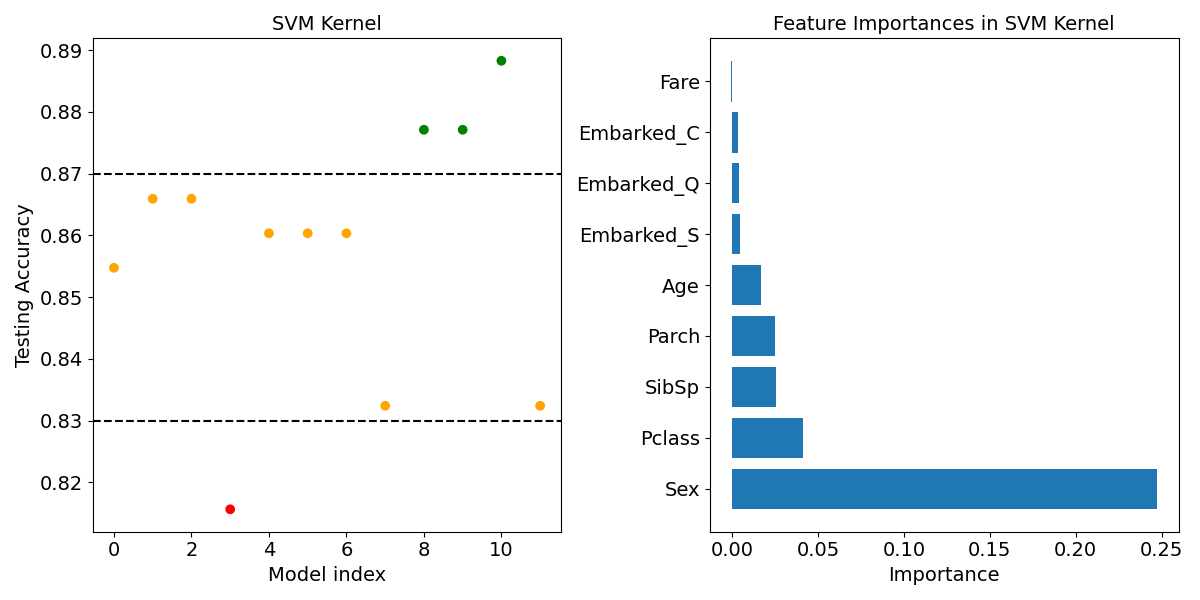
\includegraphics[width=140mm]{SVM.png}
    \caption{Performance of models of SVM kernel method}
    \label{SVM}
\end{figure} 

\begin{figure}[H]
    \centering
    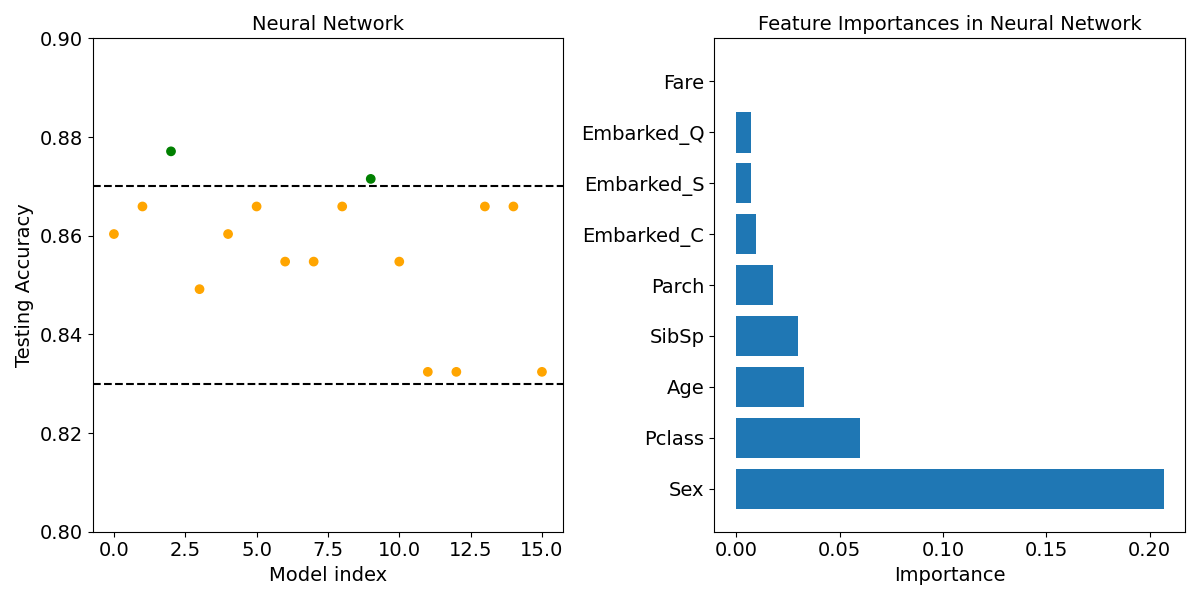
\includegraphics[width=140mm]{NN.png}
    \caption{Performance of models of the neural network method}
    \label{NN}
\end{figure} 

\begin{figure}[H]
    \centering
    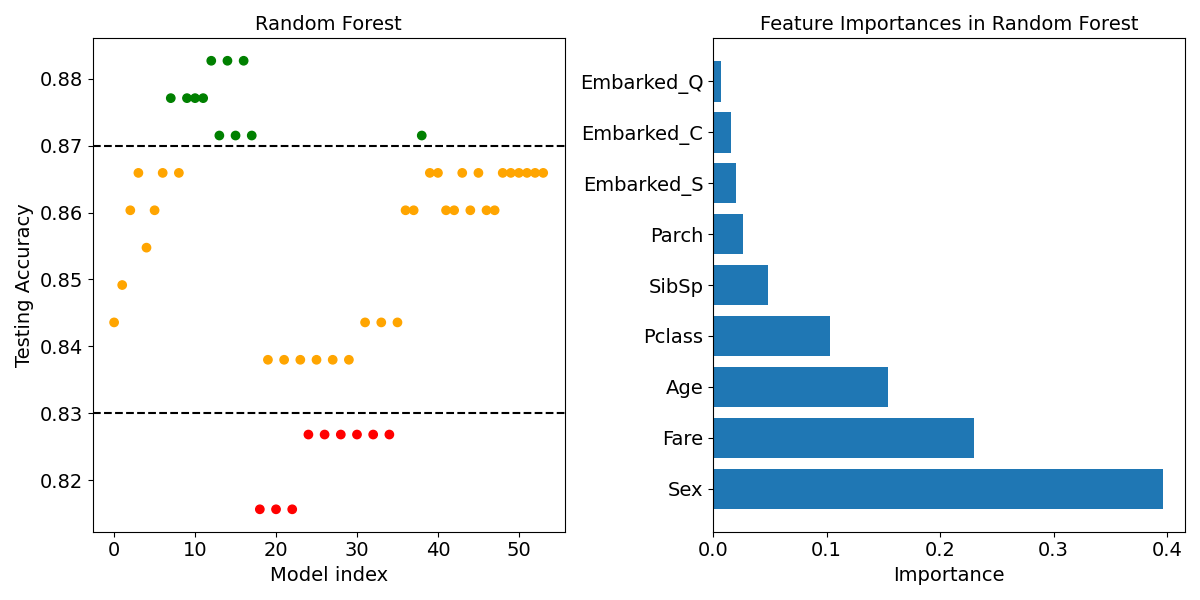
\includegraphics[width=140mm]{RF.png}
    \caption{Performance of models of the random forest method}
    \label{RF}
\end{figure} 

\section*{\textbf{Conclusion}} 
\begin{itemize}
    \item All three models performed similarly well to reach a estimated accuracy of ~88\%;
    \item In the feature importance plots in Figure 2, 3, and 4, three models share the rank 1 important feature: \textbf{Sex}, meaning \textbf{Sex} plays an important role in dictating the survival in the Titanic tragedy. However, they differ greatly on the rest of the rankings of feature importance. Most streakingly, \textbf{Fare} is the second most important feature in the random forest model, whereas it is the least in the SVM kernel method and the neutral network model.
    \item We could further improvements to the model accuracy in terms of models (try more model tuning and feature selection) and also the training data (gather more complete information or even new features for passengers).
\end{itemize}
